\begin{figure}[H]
	\centering
        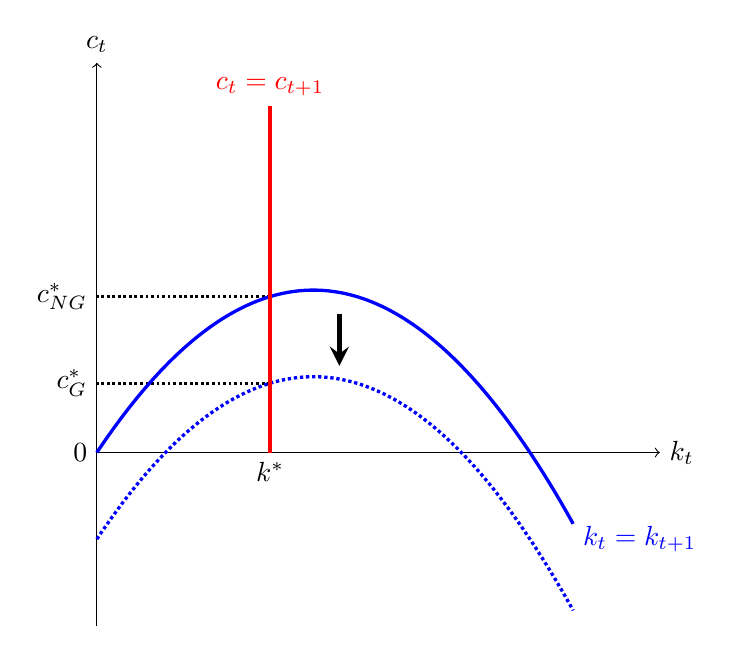
\begin{tikzpicture}[scale=1.1]
            \draw[->] (0, 0) -- (6.5, 0) node[right] {$k_{t}$};
            \draw[->] (0, -2) -- (0, 4.5) node[above] {$c_{t}$};
            % auxiliary dotted lines
            \draw[densely dotted, line width=1pt] (2,0.8) -- (0,0.8);
            \draw[densely dotted, line width=1pt] (2,1.8) -- (0,1.8);
            \node[left] at (0,0.8) {$c^{*}_{G}$};
            \node[left] at (0,1.8) {$c^{*}_{NG}$};
            % steady-state curves
            \draw[domain=0:5.5, samples=200, blue, line width = 1.2pt, variable=\x] plot ({\x}, {-0.3*\x*(\x-5)});
            \draw[domain=0:5.5, samples=200, blue, densely dotted, line width = 1.2pt, variable=\x] plot ({\x}, {-0.3*\x*(\x-5) - 1});
            \draw[red, line width=1.5pt] (2,0) -- (2,4);
            % arrow representing effect
            \draw[-stealth, line width=2pt] (2.8,1.6) -- (2.8,1);
            % imporant nodes
            \node[left] at (0,0) {$0$};
            \node[right] at (5.5,-1) {\color{blue}$k_{t} = k_{t+1}$};
            \node[above] at (2,4) {\color{red}$c_{t} = c_{t+1}$};
            \node[below] at (2,0) {$k^*$};
	\end{tikzpicture}
\end{figure}
